\documentclass[tikz, border=10pt]{standalone}
\usepackage{tikz}
\usetikzlibrary{arrows}

\begin{document}
\section*{uploaded_geometry.jpeg}
\documentclass[tikz, border=10pt]{standalone}
\usepackage{tikz}
\usetikzlibrary{arrows}


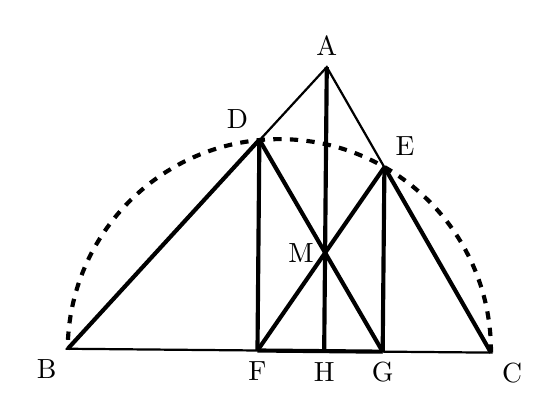
\begin{tikzpicture}[scale=1.0, >=stealth, line width=1.5pt][scale=1.0, >=stealth, line width=1.5pt]

    % === 顶点坐标 ===
    \coordinate (A) at (0.602, 1.813);
    \coordinate (B) at (-2.687, -1.764);
    \coordinate (C) at (2.687, -1.813);
    \coordinate (D) at (-0.254, 0.891);
    \coordinate (E) at (1.334, 0.542);
    \coordinate (F) at (-0.278, -1.786);
    \coordinate (G) at (1.312, -1.801);
    \coordinate (H) at (0.569, -1.794);
    \coordinate (M) at (0.581, -0.544);

    % === 以BC为直径的半圆 ===
    \draw[dashed] (C) arc (-0.5:179.5:2.688);

    % === 由图像验证得到的线段 ===
    \draw[thick] (A) -- (B) -- (C) -- cycle;

    \draw (A) -- (H);
    \draw (B) -- (D);
    \draw (C) -- (E);
    \draw (F) -- (G);

    % === 构造层：几何定义自动补全的辅助线 ===
    \draw (D) -- (F);
    \draw (E) -- (G);
    \draw (D) -- (G);
    \draw (E) -- (F);

    % === 顶点标注 ===
    \node[above] at (A) {A};
    \node[below left] at (B) {B};
    \node[below right] at (C) {C};
    \node[above left] at (D) {D};
    \node[above right] at (E) {E};
    \node[below] at (F) {F};
    \node[below] at (G) {G};
    \node[below] at (H) {H};
    \node[left] at (M) {M};

\end{tikzpicture}


\end{document}